%Introduction.TeX
\section{The Standard Model and beyond}

%Comprising 18 particles, numerous interactions between particle fields, containing many symmetries and holding a description of the fundamental interactions within nature, the Standard Model is the leading theory that describes nature with empirical evidence. This introduction's purpose is not to derive the Standard Model or show all the fundamental interactions; however, the aim is to frame the analysis conducted by briefly showcasing the Standard Model and its extension of supersymmetry with two Higgs doublet models. A table listing the particles appears below in figure \ref{fig:SM}. 



Comprising 18 particles and numerous interactions between their fields, the Standard Model provides a description of the fundamental interactions of nature.
The Standard Model (SM) which is consistent with all empirical evidence is the leading theory of the universe. 


Rather than providing a detailed description of the SM, the purpose of this introduction is to frame the analysis from a theoretical perspective.
A table listing components of the SM appears below in figure \ref{fig:SM}. 
\begin{figure}[ht!b]
  \centering
  \includegraphics[width=0.60\textwidth]{Figures/750px-Standard_Model_of_Elementary_Particles.svg.png}
  \caption{\label{fig:SM} Standard Model particles }
\end{figure}

Particles are represented by fields and interact within the theory. The simplest SM interactions of these fields are found by looking at the Dirac Lagrangian and then establishing $U(1)$ interactions that have a conserved quantity (charge). 
Noether originally proved that local transformation symmetries imply conserved currents which has extensive implications for particle physics and theories that predict quantum numbers and conserved quantities, such as charge in the $U(1)$ group ~\cite{Noether_1971}. 

After analyzing the $U(1)$ group, one typically extends the theory to include more fields and structures through higher dimensional groups. The gauge principle will be examined for $U(1)$ and then expanding to $SU(2)$ before taking the product of these groups to form the Weinberg-Salam Model.

%\subsection{Symmetry}
\section{Gauge Principle, Yang Mills Theories, and the Weinberg-Salam Model}
The gauge principle sets the stage for interactions between particle-fields in a theory. Much like in differential geometry and general relativity, there is a cost to interacting or changing through the action of a transformation. Consider the covariant derivative on a vector field $V(x)$.
\begin{equation}\mathcal{D}_\mu V(x) \equiv \text{lim}_{\Delta x^{\mu} \rightarrow 0 } \frac{V_{||}(x+\Delta x) - V(x)}{\Delta x^{\mu}} \end{equation} 
How the field changes under the transformation will determine the nature of the field. The connection terms that link the field follow from the transformation. A unitary operator can capture the parallel component in the covariant derivative. This operator carries the field and the \textit{local} transformation law depending on the symmetries and complexity of the math structure that the unitary operator carries. 
\begin{equation}V_{||}(x+\Delta x) = U(x+\Delta x)V(x+\Delta x)\end{equation}
After expanding the unitary operator, one can find the terms and phases that are carried under this transformation. 
For the $U(1)$ group, these steps give the electromagnetic field tensor and charge conservation. 
One defines the transformation and field, then works out the form of the covariant derivative and examines how the gauge field transforms ~\cite{Tully:1417476}. To put it generally
\begin{equation}
\label{eq:lt}
\Psi'= U(\overrightarrow{x})\Psi \;\;\text{particle under local transformation}\end{equation}
\begin{equation}
\label{eq:cd}
\mathcal{D}^\mu = \partial^\mu + igB^\mu \;\;\text{covariant derivative}
\end{equation}
\begin{equation}
\label{eq:gt}
B'^\mu = UB^\mu U^{-1} + \frac{i}{g}(\partial^\mu U)U^{-1} \;\;\text{gauge field transform.} 
\end{equation} 

For $U(1)$ with a unitary transformation of the form $U(x) = \exp{\frac{ie}{2}Y\cdot\beta(x)}$ 
\begin{equation}\Psi'(x)= (1+\frac{ie}{2}Y\cdot\beta(x))\Psi \;\;\text{particle field with local transformation}\end{equation}
\begin{equation}\mathcal{D}_\mu = \partial_\mu + ieA_\mu \;\;\text{covariant derivative}\end{equation}
\begin{equation}A^\mu \rightarrow A^\mu + \frac{1}{e}(\partial^\mu \beta) \;\;\text{gauge field transform.} \end{equation} 


Notably, the commutator between the covariant derivatives yields the practical field that it carries. For the $U(1) $ case, it is the electromagnetic field tensor. 
\begin{equation}  \left[ \mathcal{D}^\mu,\mathcal{D}^\nu\right] \Psi = ie F^{\mu\nu} \Psi\end{equation}

These relations are important when higher dimensional groups and more complex particle fields are considered. Yang-Mills theories take these components and analyze them under groups like $SU(2)$ or other special unitary groups. When one considers a local $SU(2)$ transformation, the terms that show up are more rich than $U(1)$.  

For $SU(2)$ with a unitary transformation of the form $U(x) = \exp{\frac{ig}{2}\bm{\tau}\cdot\bm{\alpha(x)}}$ 
\begin{equation}\Psi'(x)= (1 + \frac{ig}{2}\bm{\tau}\cdot\bm{\alpha})\Psi \;\;\text{particle field with local transformation}\end{equation}
\begin{equation}\mathcal{D}_\mu = \partial_\mu -\frac{i}{2} g \bm{\tau}\cdot \bm{W}_\mu(x) \;\;\text{covariant derivative}\end{equation}
\begin{equation}\bm{\tau}\cdot\bm{W}_\mu \rightarrow  \bm{\tau}\cdot\bm{W}_\mu + \frac{1}{g}\bm{\tau}\cdot(\partial_\mu \bm{\alpha}) - \bm{\tau}\cdot (\bm{\alpha}\times\bm{W}_\mu) \;\;\text{gauge field transform.} \end{equation}


%\begin{equation}\partial_\mu \Psi \rightarrow \partial_\mu +\frac{ig}{2}\left(\bm{\tau}\cdot\bm{\alpha}(x)\right)\partial_\mu \Psi + \frac{ig}{2}\left(\bm{\tau}\cdot\partial_\mu\bm{\alpha}(x)\right) \Psi  \end{equation}
%
%implying the covariant derivative 
%\begin{equation}\mathcal{D}_\mu = \partial_\mu -\frac{i}{2} g \bm{\tau}\cdot \bm{W}_\mu(x)\end{equation}
%Where $\bm{\tau}$ are the Pauli matrices.
%The gauge field then transforms as 
%\begin{equation}\bm{\tau}\cdot\bm{W}_\mu \rightarrow  \bm{\tau}\cdot\bm{W}_\mu + \frac{1}{g}\bm{\tau}\cdot(\partial_\mu \bm{\alpha}) - \bm{\tau}\cdot (\bm{\alpha}\times\bm{W}_\mu) \end{equation}

%Now if we consider $SU(2)\times U(1)$ and build states out of that with a coupling of only one component in the $SU(2)$ interaction then add a scalar field, the structure is there for the Weinberg-Salam Model. 
Now if we consider $SU(2)\times U(1)$ and build states out of that and add a scalar field, the structure is there for the Weinberg-Salam Model. 

\section{The Higgs Mechanism}
As mentioned in the previous section, taking the $SU(2) \times U(1)$ groups with an additional scalar field and defining their local transformations give way to the interactions within the electroweak Weinberg-Salam model. The fields transform the same way as before; however, Higgs and others thought of adding a scalar field to the theory. In order to see the interactions with the scalar field, we need to see how it transforms. 
\begin{equation}\begin{pmatrix}\phi^+ \\ \phi^0\end{pmatrix} = \frac{1}{\sqrt{2}}\begin{pmatrix} \phi_3 + i\phi_4 \\ \phi_3 + i\phi_4\end{pmatrix}  \end{equation}
This scalar field transforms in the following way under $U(1)$ and $SU(2)$ transformations 
\begin{equation}\begin{pmatrix}\phi^+ \\ \phi^0\end{pmatrix} \rightarrow \begin{pmatrix} e^{ig\frac{\beta}{2}} & 0 \\ 0 & e^{ig\frac{\beta}{2}}\end{pmatrix}\begin{pmatrix}\phi^+ \\ \phi^0\end{pmatrix} \; U(1) \end{equation}
\begin{equation}\begin{pmatrix}\phi^+ \\ \phi^0\end{pmatrix} \rightarrow e^{\frac{ig}{2}\bold{\tau}\cdot\bold{\alpha}}    \begin{pmatrix}\phi^+ \\ \phi^0\end{pmatrix} \; SU(2) \end{equation}
\begin{equation}\mathcal{D}_\mu \phi = \partial_\mu \phi - \frac{i}{2}g\bold{\tau}\cdot\bold{W}_\mu \phi - \frac{i}{2}g'B_\mu\phi \text{,}\end{equation}
yielding the Higgs field Lagrangian component 
\begin{equation}\mathcal{L} = (\mathcal{D}^\mu \phi)^\dag (\mathcal{D}_\mu \phi) + \frac{m^2_h}{2}\phi^\dag \phi - \frac{\lambda}{4}(\phi^\dag\phi)^2 \text{.}\end{equation} 
The Higgs potential contains the typical ``Mexican hat" shape. The kinetic term holds interesting interactions and implications for the gauge bosons in the theory. 
All together the Weinberg-Salam model with the Higgs field is (with $L$ and $R$ being lefthanded and righthanded fermion fields) ~\cite{Lancaster:1629337}
\begin{align}
\label{eq:ws}
\mathcal{L} &= \bar{L}i \gamma^\mu \mathcal{D}_\mu L +\bar{R}i \gamma^\mu \mathcal{D}_\mu R + (\mathcal{D}^\mu \phi)^\dag(\mathcal{D}_\mu\phi)  \\
            &+\frac{m^2_h}{2}\phi^\dag \phi - \frac{\lambda}{4}(\phi^\dag\phi)^2 - G_e(\bar{L}\phi R +\bar{R}\phi^\dag L)\nonumber \\
            &-\frac{1}{4}G^{(W)}_{\mu\nu}\cdot G^{(W)\mu\nu} - \frac{1}{4}F^{(B)}_{\mu\nu} F^{(B)\mu\nu}    \text{.} 
\end{align}

The Weinberg-Salam Model has major implications: the terms $L$ and $R$ along with their hermitian conjugates form an interaction with the Higgs field giving these fermions mass. 
This equation, along with the shape of the Higgs potential, imply spontaneous symmetry breaking and interactions that produce massive vector gauge bosons and massless photons. 

\section{Higgs Doublet Models}
The Standard Model can naturally be extended by giving more complexity to the fields. 
%In order to extend beyond the standard model, a natural place to start is giving more complexity to the fields. 
Suppose that there were multiple scalar fields instead of just the single Higgs field $\phi$. Then one can consider adding another component, thus making it a doublet. Adding the doublet, and working out the relations for the field, creates the most general two-Higgs doublet model (2HDM) with the Higgs potential shown in equation \ref{eq:2hd} ~\cite{Branco_2012}.
\begin{align} 
\label{eq:2hd}
V &= m^2_1|H_1|^2 + m^2_2|H_2|^2 + \frac{\lambda_1}{2}|H_1|^2 + \frac{\lambda_2}{2}|H_2|^2  \\
    &+\lambda_3|H_1|^2|H_2|^2 + \lambda_4|H^\dag_1 H_2|^2 \nonumber \\
    &+\frac{\lambda_5}{2}\left((H_1H_2)^2 + c.c.\right) +m^2_{12}\left(H_1 H_2 + c.c.\right) \nonumber \\
    &+\left(\lambda_6|H_1|^2(H_1 H_2) + c.c.\right) \nonumber \\
    &+\left(\lambda_7|H_2|^2(H_1 H_2) + c.c.\right) \nonumber 
\end{align}

Expanding around the minimum of the potential yields two doublets with vacuum expectation values $v_1$ and $v_2$. They are usually mixed under a rotation parameter $\tan \beta = v_1 / v_2$. After one carries out the interactions with the SM gauge bosons which consume the complex field components and a neutral pseudoscalar combination of scalar Higgs field components, the surviving three real degrees of freedom yield one neutral pseudoscalar mass eigenstate along with two neutral scalar mass eigenstates. $A$ denotes the pseudoscalar, $h$ the lighter neutral SM like Higgs, and $H^0$ the remaining scalar. As with the notation for fields that interact with the potential, the rotation matrix that mixes these scalars into the components that interact under the potential is parametrized by the continuous parameter $\alpha$ 
\begin{equation}
\begin{pmatrix} h \\ H^0\end{pmatrix} = \begin{pmatrix} -\sin\alpha & \cos\alpha \\ \cos\alpha & \sin\alpha \end{pmatrix}   \begin{pmatrix}H^0_{1,R} \\ H^0_{2,R}\end{pmatrix} 
\end{equation}.


In the literature this parameter is important because $\tan \beta$ and $\alpha$ set the possible couplings to SM particles. Next, if a complex scalar singlet is added, couplings to SM fermions and bosons are supported ~\cite{Curtin_2014}.
\begin{equation}S = \frac{1}{\sqrt{2}}(S_R + iS_I)\end{equation}

The scalar singlet doesn't have Yukawa couplings, but rather couples to $H_{1,2}$. Through its mixing with $H_{1,2}$ the singlet can couple to SM fermions. 

A possible coupling that preserves the SM Higgs by keeping $\theta_a$ small could be defined as  
\begin{equation}a \equiv \cos \theta_a S_i + \sin \theta_a A ,\;\; \theta_a << 1 \end{equation}

This allows for decays like $h\rightarrow aa \rightarrow X\bar{X}Y\bar{Y}$, where $X$ and $Y$ are SM fermions or bosons. Looking into the phase space where the mixing is small frames the Higgs pseudoscalar analysis in a region with little SM resonance---making it also a general search for any beyond SM (BSM) phenomena.
There are terms in the effective Lagrangian that support the $h \rightarrow aa $ decays:
\begin{align}
\label{eq:efflag}
\mathcal{L} &\subset g_{hAA}hAA + \lambda_S|S^2|^2  \\
            &\subset g_{hAA}\sin^2\theta_a haa + 4\lambda_S v_s \sin{\zeta_1} \cos^2\theta_a haa \nonumber 
\end{align}
here $\zeta$ is just the angle that mixes the singlet with the SM Higgs (needed because of the added state). These interactions give rise to different scenarios that favor certain SM fermions and bosons. According the literature, four distinct scenarios are typically entertained.  The scenarios, supported by the effective Lagrangian \ref{eq:efflag}, yield branching fractions as a function of $a$-mass and $\tan\beta$.  These are enumerated below:
\begin{itemize}
\item Type I: Fermions couple only to the $H_2$ field and are independent of $\tan\beta$, pseudoscalar coupling are proportional to the SM Higgs (final state of the fermions) represented in figure \ref{fig:br2HDM-1}.
\item Type II: Down-type fermions are particularly favored supporting more NMSSM models and is dependent on $\tan\beta$ represented in figure \ref{fig:br2HDM-2}. 
\item Type III: Branching ratios are directly dependent on $\tan\beta$ and are emphasized when more than one lepton is considered. $\tau^+ \tau^-$ can dominate in this scenario represented in figure \ref{fig:br2HDM-3}. 
\item Type IV: Dependent on $\tan\beta$, for $\tan \beta < 1 $, branching ratios for $b\bar{b}$, $c\bar{c}$, and $\tau^+ \tau^-$ are similar (supports $2b2\tau$) represented in figure \ref{fig:br2HDM-4}.
\end{itemize}


\begin{figure}[ht!b]
  \centering
\includegraphics[width=0.9\textwidth]{aToSMvsaMass_type1.png}           \\
    \caption{\label{fig:br2HDM-1} Type I 2HDM+S scenario branching fractions ~\cite{Branco_2012}}
\end{figure}

\begin{figure}[ht!b]
  \centering
\includegraphics[width=0.9\textwidth]{aToSMvsaMass_type2_tbeta0.5.png}
\includegraphics[width=0.9\textwidth]{aToSMvsaMass_type2_tbeta5.png}           \\
    \caption{\label{fig:br2HDM-2} Type II 2HDM+S scenario branching fractions ~\cite{Branco_2012}}
\end{figure}

\begin{figure}[ht!b]
  \centering
\includegraphics[width=0.9\textwidth]{aToSMvsaMass_type3_tbeta0.5.png}
\includegraphics[width=0.9\textwidth]{aToSMvsaMass_type3_tbeta5.png}           \\
    \caption{\label{fig:br2HDM-3} Type III 2HDM+S scenario branching fractions ~\cite{Branco_2012}}
\end{figure}



\begin{figure}[ht!b]
  \centering
\includegraphics[width=0.9\textwidth]{aToSMvsaMass_type4_tbeta0.5.png}
\includegraphics[width=0.9\textwidth]{aToSMvsaMass_type4_tbeta5.png}           \\
    \caption{\label{fig:br2HDM-4} Type IV 2HDM+S scenario branching fractions ~\cite{Branco_2012}}
\end{figure}

\section{Previous and present searches in 2HDM+S models}

%Due to the Nature of the Electroweak Symmetry Breaking Mechanism ~\cite{Englert:1964et,Higgs:1964ia,Higgs:1964pj,Guralnik:1964eu,Higgs:1966ev,Kibble:1967sv}, the Higgs couples to all Standard Model particles.
As shown in the previous section, the Higgs couples to all massive SM particles and also to new particles provided that the new particles have mass.  
BSM theories contain ample room for the Higgs to couple to new particles, making the Higgs an excellent window to investigate any physics beyond the SM.
Notably, the two Higgs doublet model (2HDM) with its extension of a scalar singlet is considered (2HDM+S).
These types of BSM theories can solve the $\mu$ coupling problem in Super Symmetry (SUSY), while maintaining general support of SUSY (Holomorphy), Axion-like Models (Peccei-Quinn), electroweak baryogensis and several Grand Unified Theories (GUTs) ~\cite{Branco_2012}.

A representative diagram showing the physics process and the branching ratio as a function of $\text{tan}\beta$ is shown in figure \ref{fig:feynman_haa}. This pseudoscalar Higgs search for ``resolved" $a$ particles in the range of $20$ to $60$ GeV is a good search for new physics.
In 2016 this general search was carried out with 35.9 $\text{fb}^{-1}$ of data, and new competitive limits were set in reference ~\cite{CMS-HIG-17-029}.

Given the potential for improvements in the limits for different 2HDM+S types, extending this search using the full RunII dataset is motivated. 


\begin{figure}[ht!b]
  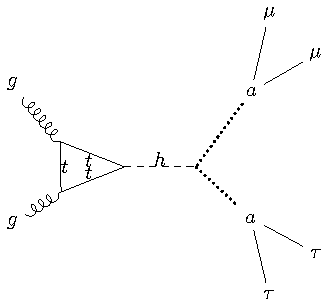
\includegraphics[width=0.47\textwidth]{Figures/feynman_haa.pdf}
  \includegraphics[width=0.47\textwidth]{Figures/2m2t_BR_a40_t1-4.png}\\
    \caption{\label{fig:feynman_haa} Diagram of Higgs decay to pseudoscalar $a$ particles (Left) and branching ratios for pseudoscalar production in different $\text{tan}\beta$ scenarios and different 2HDM+S Types (right)}
\end{figure}

The branching ratios change based on the function of $\text{tan}\beta$ depending on the type of model under investigation. In particular, we look at types I-IV. Type III is expected to be most sensitive as it maintains a larger branching ratio compared to other decay modes over the range of the pseudoscalar masses when focusing on the final state of two muons and two tau leptons. In addition to the search for this model, any deviation from the SM prediction in the effective mass range would also be found.

